\documentclass[tikz, border=0mm]{standalone}
\usetikzlibrary{calc}
\newcommand{\tikzsetnextfilename}[1]{}


% One style for all polyomino outlines (adjust to taste)
\tikzset{
  polyoutline/.style={draw=black, line width=2pt}
}

% (3): horizontal bar of length 3
% cells: (0,0), (1,0), (2,0)
\newcommand{\shapeH}[2]{%
  \begin{scope}[shift={(#1,#2)}]
    \draw[polyoutline]
      (0,0) -- (3,0) -- (3,1) -- (0,1) -- cycle;
  \end{scope}%
}

% (1,1,1): vertical bar of length 3
% cells: (0,0), (0,1), (0,2)
\newcommand{\shapeI}[2]{%
  \begin{scope}[shift={(#1,#2)}]
    \draw[polyoutline]
      (0,1) -- (1,1) -- (1,-2) -- (0,-2) -- cycle;
  \end{scope}%
}

% (2,1): hook shape
% cells: (0,0), (1,0), (0,1)
\newcommand{\shapeL}[2]{%
  \begin{scope}[shift={(#1,#2)}]
    \draw[polyoutline]
      (0,-1) -- (2,-1) -- (2,0) -- (1,0) -- (1,1) -- (0,1) -- cycle;
  \end{scope}%
}

% (2,2)/(1): skew shape
% cells: (0,0), (1,0), (1,1)
\newcommand{\shapeS}[2]{%
  \begin{scope}[shift={(#1,#2)}]
    \draw[polyoutline]
      (0,1) -- (2,1) -- (2,-1) -- (1,-1) -- (1,0) -- (0,0) -- cycle;
  \end{scope}%
}


\begin{document}

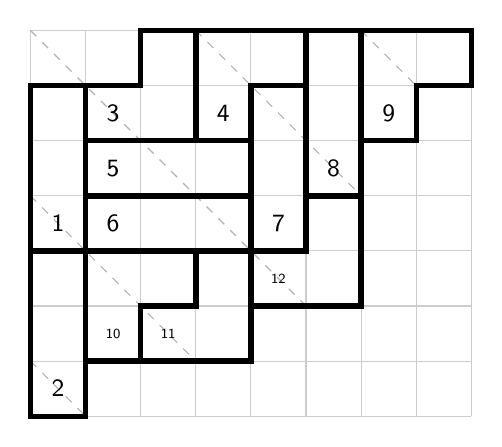
\begin{tikzpicture}[xscale=0.7,yscale=-0.7]

  % --- styles ---
  \tikzset{
    gridbg/.style={draw=gray!40, line width=0.4pt},
    trioutline/.style={draw=black, line width=1.2pt},
    diag/.style={draw=gray!60, dashed},
  }

  % --- background & grid ---
  \draw[step=1,gridbg] (0,0) grid (8,7);

  % =========================
  %  OPTIONAL DIAGONALS
  % =========================

  \draw[diag] (0,0) -- (5,5);
  \draw[diag] (0,3) -- (3,6);
  \draw[diag] (0,6) -- (1,7);
  \draw[diag] (3,0) -- (6,3);
  \draw[diag] (6,0) -- (7,1);




  % =========================
  %  OUTLINED POLYOMINOES
  % =========================

    \shapeI{0}{3}
    \shapeI{0}{6}
    \shapeS{1}{1}
    \shapeL{3}{1}
    \shapeH{1}{2}
    \shapeH{1}{3}
    \shapeI{4}{3}
    \shapeI{5}{2}
    \shapeL{6}{1}
    \shapeL{1}{5}
    \shapeS{2}{5}
    \shapeS{4}{4}

\begin{scope}[shift={(0.5,0.5)}]
  \node[font=\sffamily\small] at (0,3) {1};
  \node[font=\sffamily\small] at (0,6) {2};

  \node[font=\sffamily\small] at (1,1) {3};
  \node[font=\sffamily\small] at (3,1) {4};

  \node[font=\sffamily\small] at (1,2) {5};
  \node[font=\sffamily\small] at (1,3) {6};

  \node[font=\sffamily\small] at (4,3) {7};
  \node[font=\sffamily\small] at (5,2) {8};
  \node[font=\sffamily\small] at (6,1) {9};

  \node[font=\sffamily\tiny]  at (1,5) {10};
  \node[font=\sffamily\tiny]  at (2,5) {11};
  \node[font=\sffamily\tiny]  at (4,4) {12};
\end{scope}



\end{tikzpicture}


%
% \begin{tikzpicture}[scale=0.7]
%   % We work on a 7x7 grid of unit squares
%   % x = 0..7 (columns), y = 0..7 (rows), bottom-left is (0,0)
%
%   % styles
%   \tikzset{
%     gridline/.style={draw=black, line width=0.6pt},
%     diag/.style={draw=gray!60, dashed},
%   }
%
%
%   % full grid (you can make these lighter if you want)
%   \draw[step=1,gray!40] (0,0) grid (7,7);
%   % outer frame (optional, slightly thicker)
%   \draw[gridline] (0,0) rectangle (7,7);
%
%   % dashed diagonals, translated from the SVG coordinates to grid coords
%   % (just the same pattern, but in integer grid units)
%   \draw[diag] (0,1) -- (1,0);
%   \draw[diag] (0,3) -- (3,0);
%   \draw[diag] (0,7) -- (7,0);
%   \draw[diag] (3,7) -- (7,3);
%   \draw[diag] (6,7) -- (7,6);
%
%   % Labels: each number sits at the center of its square (c,r)
%   % (c = column index, r = row index, with r=0 at bottom)
%
%   % helper macro: place text at center of cell (c,r)
%   \newcommand{\celllabel}[3][]{%
%     \node[font=\sffamily\small,#1] at (#2+0.5,#3+0.5) {#1};%
%   }
%
%   % But it's cleaner to just write nodes directly:
%   \node[font=\sffamily\small] at (0+0.5,3+0.5) {1};
%   \node[font=\sffamily\small] at (0+0.5,6+0.5) {2};
%   \node[font=\sffamily\small] at (1+0.5,5+0.5) {3};
%   \node[font=\sffamily\small] at (3+0.5,5+0.5) {4};
%   \node[font=\sffamily\small] at (1+0.5,4+0.5) {5};
%   \node[font=\sffamily\small] at (1+0.5,3+0.5) {6};
%   \node[font=\sffamily\small] at (4+0.5,3+0.5) {7};
%   \node[font=\sffamily\small] at (5+0.5,4+0.5) {8};
%   \node[font=\sffamily\small] at (6+0.5,5+0.5) {9};
%
%   % 10, 11, 12 (originally smaller font — you can use \tiny if you like)
%   \node[font=\sffamily\tiny] at (1+0.5,1+0.5) {10};
%   \node[font=\sffamily\tiny] at (2+0.5,1+0.5) {11};
%   \node[font=\sffamily\tiny] at (4+0.5,2+0.5) {12};
%
% \end{tikzpicture}



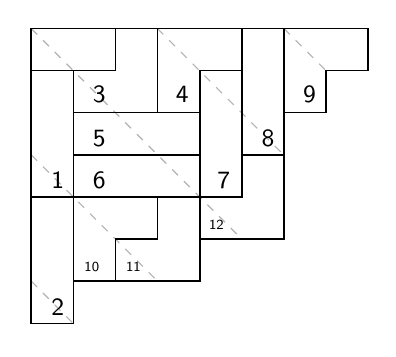
\begin{tikzpicture}[x=1pt,y=-1pt]
  % overall canvas
  \useasboundingbox (0,0) rectangle (123,109);

  % styles
  \tikzset{
    g0/.style={draw=gray!60,dashed,line cap=butt,line join=miter},
    g1/.style={draw=black,line width=0.6pt,line cap=butt,line join=miter},
  }

  % white background
  \fill[white] (0,0) rectangle (123,109);

  % gray dashed “diagonals”
  \draw[g0] (1.3, 91.6) -- ++(15.2,15.3);
  \draw[g0] (1.3, 46.0) -- (46.9,91.6);
  \draw[g0] (1.3,  0.3) -- (77.4,76.4);
  \draw[g0] (46.9, 0.3) -- (92.6,46.0);
  \draw[g0] (92.6, 0.3) -- ++(15.2,15.2);

  % --- black polygonal structure (split into simpler pieces) ---

  % left column: three stacked blocks
  \draw[g1] (1.3,  0.3) -- (31.7, 0.3) -- (31.7,15.5) -- (1.3,15.5) -- cycle;
  \draw[g1] (1.3, 15.5) -- (16.5,15.5) -- (16.5,61.2) -- (1.3,61.2) -- cycle;
  \draw[g1] (1.3, 61.2) -- (16.5,61.2) -- (16.5,106.9) -- (1.3,106.9) -- cycle;

  % “L” shaped region around (31.7,0.3)
  \draw[g1]
    (31.7, 0.3) -- (46.9, 0.3) -- (46.9,30.7) --
    (16.5,30.7) -- (16.5,15.5) -- (31.7,15.5) -- cycle;

  % middle block under that
  \draw[g1]
    (46.9, 0.3) -- (77.4, 0.3) -- (77.4,15.5) --
    (62.2,15.5) -- (62.2,30.7) -- (46.9,30.7) -- cycle;

  % central rectangles
  \draw[g1] (16.5,30.7) -- (62.2,30.7) -- (62.2,46.0) -- (16.5,46.0) -- cycle;
  \draw[g1] (16.5,46.0) -- (62.2,46.0) -- (62.2,61.2) -- (16.5,61.2) -- cycle;
  \draw[g1] (62.2,15.5) -- (77.4,15.5) -- (77.4,61.2) -- (62.2,61.2) -- cycle;

  % right vertical blocks
  \draw[g1] (77.4, 0.3) -- (92.6, 0.3) -- (92.6,46.0) -- (77.4,46.0) -- cycle;
  \draw[g1]
    (92.6, 0.3) -- (123.0, 0.3) -- (123.0,15.5) --
    (107.8,15.5) -- (107.8,30.7) -- (92.6,30.7) -- cycle;

  % lower central “steps”
  \draw[g1]
    (16.5,61.2) -- (46.9,61.2) -- (46.9,76.4) --
    (31.7,76.4) -- (31.7,91.6) -- (16.5,91.6) -- cycle;

  \draw[g1]
    (46.9,61.2) -- (62.2,61.2) -- (62.2,91.6) --
    (31.7,91.6) -- (31.7,76.4) -- (46.9,76.4) -- cycle;

  \draw[g1]
    (77.4,46.0) -- (92.6,46.0) -- (92.6,76.4) --
    (62.2,76.4) -- (62.2,61.2) -- (77.4,61.2) -- cycle;


  \node[font=\sffamily\small,anchor=base west] at ( 5, 58) {1};
  \node[font=\sffamily\small,anchor=base west] at ( 5,104) {2};
  \node[font=\sffamily\small,anchor=base west] at (20, 27) {3};
  \node[font=\sffamily\small,anchor=base west] at (50, 27) {4};
  \node[font=\sffamily\small,anchor=base west] at (20, 43) {5};
  \node[font=\sffamily\small,anchor=base west] at (20, 58) {6};
  \node[font=\sffamily\small,anchor=base west] at (65, 58) {7};
  \node[font=\sffamily\small,anchor=base west] at (81, 43) {8};
  \node[font=\sffamily\small,anchor=base west] at (96, 27) {9};

  \node[font=\sffamily\tiny,anchor=base west] at (17, 88) {10};
  \node[font=\sffamily\tiny,anchor=base west] at (32, 88) {11};
  \node[font=\sffamily\tiny,anchor=base west] at (62, 73) {12};
\end{tikzpicture}


\end{document}
